\begin{problem}{문자열 게임}{표준 입력(stdin)}{표준 출력(stdout)}{1\,초}{512\,MB}

건덕이는 문자가 일렬로 적혀있는 보드에서 게임을 하고 있다. 보드에는 $N$ 개의 알파벳 대문자가 나란히 적혀있다. 건덕이는 또 다른 $M$ 자리 영어 단어를 가지고 게임을 진행한다.

우선 보드의 한 지점에서 첫 번째 문자가 보드의 문자와 일치하는지 확인한다.
L(왼쪽) 또는 R(오른쪽) 방향으로 이동한 후에 다음 문자와 보드의 문자가 일치하는지 확인한다.
건덕이가 가지고 있는 문장이 종료하면 총 매칭된 문자의 개수를 확인한다.

예를 들어, 보드에 "KONKUK" 이라는 문자가 적혀있고, "KONDUCK" 이라는 단어로 게임을 시작한다면, 2번째 문자부터 RRRRLL 순으로 이동한다면 마지막 1개의 문자만이 매칭된다. 가장 많은 문자와 매칭하기 위해서는 1번째 문자부터 RRRRLR 순으로 이동하여 4개의 문자가 매칭되는 경우이다.

\begin{center}
  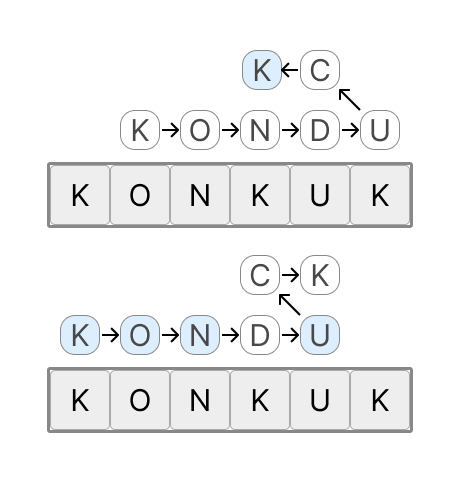
\includegraphics[width=0.4\textwidth]{../pictures/image.png} \\
\end{center}

보드와 가지고 있는 단어가 주어졌을 때, 건덕이가 얻을 수 있는 최대 점수를 구하는 프로그램을 작성해보자.

\InputFile
첫째 줄에 보드의 길이와 건덕이가 가지고 있는 문자열의 길이를 나타내는 정수 $N, M$이 공백으로 구분되어 주어진다. $( 2 \le N, M \le 5\,000 )$

둘째 줄에는 보드의 문자가 순서대로 주어진다.

셋째 줄에는 가지고 있는 문자열이 주어진다.

이때, 두 문자열은 모두 알파벳 대문자로만 구성되어 있다.

\OutputFile
첫째 줄에 최대 매칭 횟수를 출력한다.

\Examples

\begin{example}
\exmp{
6 7
KONKUK
KONDUCK
}{%
4
}%
\exmp{
2 7
AB
AAAAAAA
}{%
4
}%
\exmp{
3 10
AAA
HELLOWORLD
}{%
0
}%
\end{example}

\Note
Python3 를 이용하면 시간 초과가 될 수 있으니, PyPy3 를 이용해 주시기 바랍니다.
\end{problem}
